\documentclass{beamer}
\usetheme{Madrid}

\usepackage{amsmath, amssymb, amsthm}
\usepackage{graphicx}
\usepackage{listings}
\usepackage[utf8]{inputenc}
\usepackage{hyperref}

\title{9.1.5}
\author{EE24BTECH11004 - Ankit Jainar}
\date{}

\begin{document}

\frame{\titlepage}

\begin{frame}
\frametitle{Question}
Solve the differential equation:
\begin{align*}
    \frac{d^2y}{dx^2} = \cos(3x) + \sin(3x)
\end{align*}
\end{frame}

\begin{frame}
\frametitle{Solution: Theoretical Approach}
Given:
\begin{align}
    \frac{d^2y}{dx^2} &= \cos(3x) + \sin(3x)
\end{align}
Integrating both sides:
\begin{align}
    \frac{dy}{dx} &= \int \cos(3x) dx + \int \sin(3x) dx + c_1 \\
    &= \frac{\sin(3x)}{3} - \frac{\cos(3x)}{3} + c_1
\end{align}
\newline
Integrating again:
\begin{align}
    y &= \int \left( \frac{\sin(3x)}{3} - \frac{\cos(3x)}{3} + c_1 \right) dx + c_2 \\
    &= -\frac{\cos(3x)}{9} - \frac{\sin(3x)}{9} + c_1x + c_2
\end{align}
\end{frame}

\begin{frame}
\frametitle{Solution: Theoretical Approach (contd.)}
Assuming the initial conditions:
\begin{itemize}
    \item $y(0) = 0$
    \item $y'(0) = 0$
\end{itemize}
\newline
Substituting $y(0) = 0$:
\begin{align}
    -\frac{\cos(0)}{9} - \frac{\sin(0)}{9} + c_1 \cdot 0 + c_2 &= 0 \\
    c_2 &= \frac{1}{9}
\end{align}
Substituting $y'(0) = 0$:
\begin{align}
    \frac{\sin(0)}{3} - \frac{\cos(0)}{3} + c_1 &= 0 \\
    c_1 &= \frac{1}{3}
\end{align}
Thus, the solution is:
\begin{align}
    y(x) = -\frac{\cos(3x)}{9} - \frac{\sin(3x)}{9} + \frac{x}{3} + \frac{1}{9}
\end{align}
\end{frame}

\begin{frame}
\frametitle{Solution: Computational Approach}
The given differential equation is:
\begin{align}
    \frac{d^2y}{dx^2} = \cos(3x) + \sin(3x)
\end{align}
Using discretization, the second-order derivative can be approximated as:
\begin{align}
    y''(t+h) = y''(t) + h \cdot \left( \cos(3t) + \sin(3t) \right)
\end{align}
\end{frame}

\begin{frame}
\frametitle{Solution: Computational Approach (contd.)}
Expressing this as a system of equations:
\begin{align}
    \vec{y}_{k+1} = 
    \begin{bmatrix}
        1 & h & \frac{h^2}{2} \\
        0 & 1 & h \\
        0 & 0 & 1
    \end{bmatrix} 
    \cdot 
    \vec{y}_k + 
    \begin{bmatrix}
        0 \\
        0 \\
        h^2 \left( \cos(3x_k) + \sin(3x_k) \right)
    \end{bmatrix}
\end{align}
By iterating over time steps, the computational solution is computed.
\newline
Comparison between the theoretical and computational solutions is shown below.
\end{frame}

\begin{frame}
\frametitle{Comparison of Results}
\begin{figure}[h!]
    \centering
    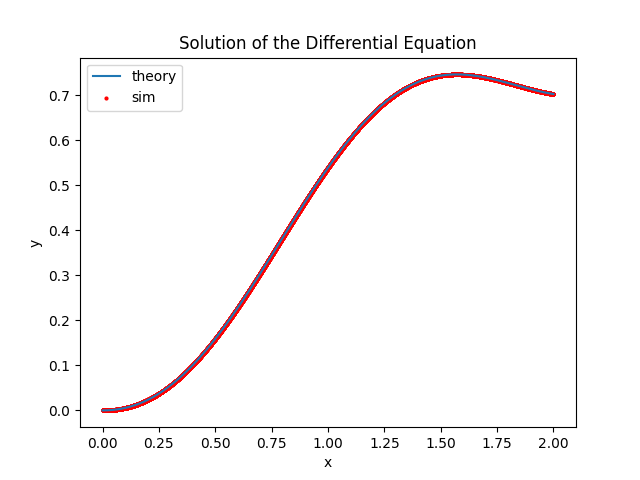
\includegraphics[width=\columnwidth]{figs/fig1.png} % Replace with your plot file
    \caption{Comparison of $y(x)$: Theoretical vs Computational}
    \label{comparison}
\end{figure}
\end{frame}
\begin{frame}{allowframebreaks}
\frametitle{C-Code}
\begin{figure}[ht]
                        \centering
                        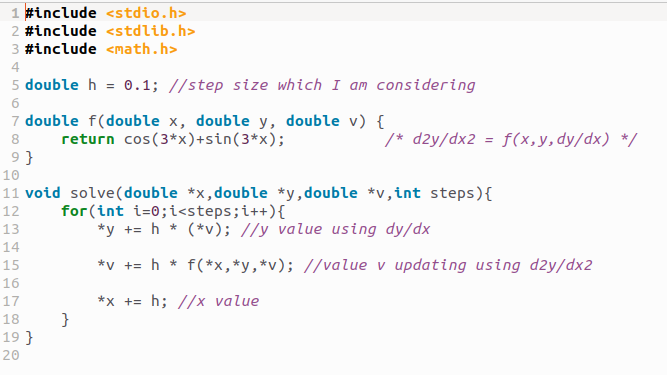
\includegraphics[width=\columnwidth]{figs/fig2.png}
                        \
\end{figure}
\end{frame}

\begin{frame}{allowframebreaks}
\frametitle{Code for plot}
\begin{figure}[ht]
                        \centering
                        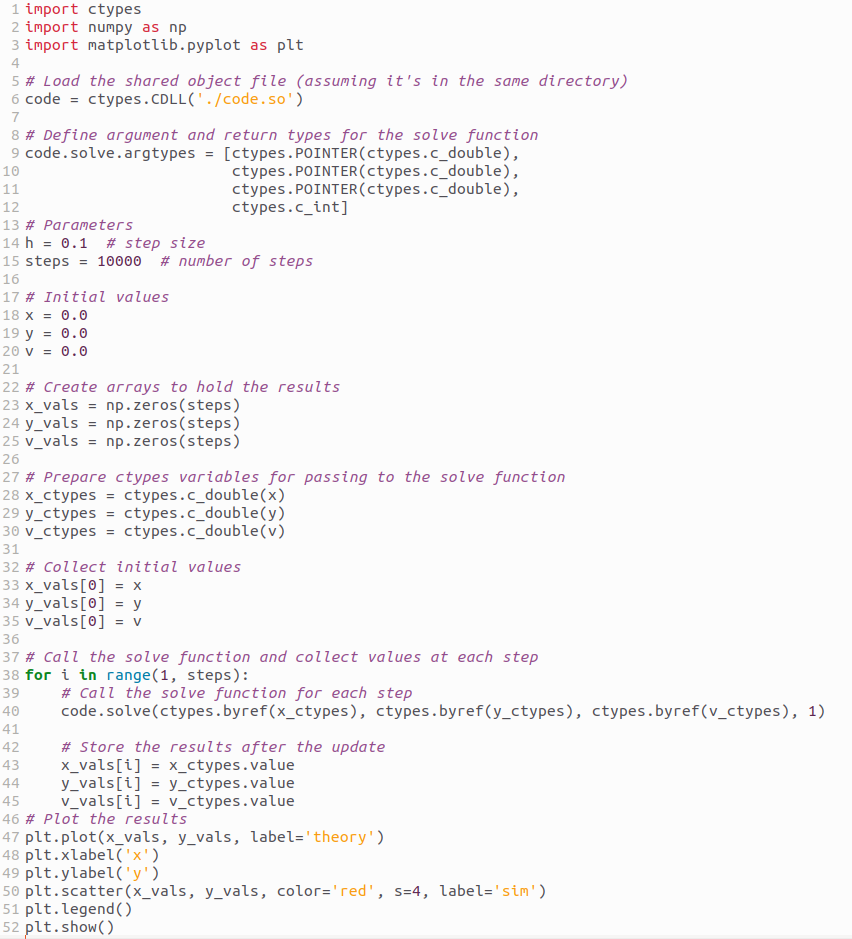
\includegraphics[width=6cm, height=8cm]{figs/fig3.png}

                        
\end{figure}
\end{frame}


\end{document}

